\setlength{\fboxsep}{4.5pt}
\noindent\fcolorbox{gray}{white}{\parbox{\fboxwidth}{
		\begin{wrapfigure}[6]{r}{0.47\textwidth}
			\begin{center}
				\vspace{-1.3em}
				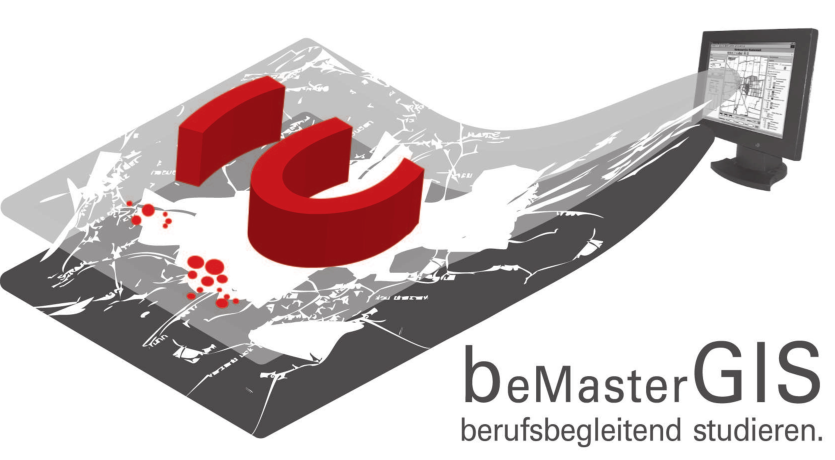
\includegraphics[width=\linewidth]{210_beMasterGIS_final}
				%		\vspace{-2em}
			\end{center}
		\end{wrapfigure}
		\textbf{Bronzesponsor}\\
		Mit dem online-ge\-stütz\-tem Fernstudiengang zum Mas\-ter Geo\-in\-for\-mations\-sys\-teme (Master of Engineering) 
		an der Hochschule Anhalt am Campus Dessau -- haben Fachanwender von Geoinformationssystemen (GIS) 
		die Chance Ihr Fachwissen entsprechend zu erweitern. Zielgruppe sind Anwender von 
		Geoinformationssystemen, die in der kommunalen Verwaltung, 
		im Planungsbereich, im Umwelt- und Naturschutz, in der 
		Versorgungswirtschaft, im Marketing und anderen Bereichen arbeiten oder die Verbindung mit 
		GIS mit ihrem persönlichen Arbeitsumfeld planen. Das berufsbegleitende fünfsemestrige Fernstudium 
		entspricht in Qualität, Umfang und Wertigkeit einem Direktstudium, es  kommt mit wenigen 
		Präsenzphasen aus, bis zu zwei Semester sind für die Anfertigung der Masterthesis vorgesehen.
			}
		}
		\setlength{\fboxsep}{3pt}